\documentclass[12pt, a4paper]{report}
\usepackage{graphicx, array, amsthm, amssymb, amsmath, algorithm, algpseudocode, float, xcolor, thmtools, thmbox, chronology,multirow,tikz}
\usepackage[english]{babel}

\makeatletter
\renewcommand\thmbox@headstyle[2]{\bfseries #1}
\makeatother
\newtheorem[style=M,bodystyle=\normalfont]{theorem}{Theorem}
\newtheorem[style=M,bodystyle=\normalfont]{corollary}{Corollary}
\newtheorem[style=M,bodystyle=\normalfont]{lemma}{Lemma}
\newtheorem[style=M,bodystyle=\normalfont]{definition}{Definition}
\newcommand{\tikzxmark}{%
\tikz[scale=0.23] {
    \draw[line width=0.7,line cap=round] (0,0) to [bend left=6] (1,1);
    \draw[line width=0.7,line cap=round] (0.2,0.95) to [bend right=3] (0.8,0.05);
}}


\title{Data Bases II \\ \textit{Theory}}
\author{Christian Rossi}
\date{Academic Year 2023-2024}

\begin{document}

\maketitle

\newpage

\begin{abstract}
    The course aims to prepare software designers on the effective development of database applications. First, the course presents the fundamental features of current database 
    architectures, with a specific emphasis on the concept of transaction and its realization in centralized and distributed systems. Then, the course illustrates the main directions 
    in the evolution of database systems, presenting approaches that go beyond the relational model, like active databases, object systems and XML data management solutions.
\end{abstract}

\newpage

\tableofcontents

\newpage

\chapter{Introduction}
    \section{Data Base Management System}
    \begin{definition}
        A \emph{Data Base Management System} is a software product capable of managing data collections that are: 
        \begin{itemize}
            \item Large: much larger than the central memory available on the computers that run the software. 
            \item Persistent: with a lifetime which is independent of single executions of the programs that access them. 
            \item Shared: used by several applications at a time. 
            \item Reliable: ensuring tolerance to hardware and software failures. 
            \item Data ownership respectful: by disciplining and controlling accesses. 
        \end{itemize}
    \end{definition}
    \begin{chronology}[5]{1990}{2020}{\textwidth}
        \event{1992}{SQL '92}
        \event{1999}{SQL '99}
        \event{2001}{Ranking in databases}
        \event{2003}{XML-related features}
        \event{2005}{NoSQL}
        \event{2006}{X-Query}
        \event{2009}{JPA final release}
        \event{2011}{Temporal databases}
        \event{2016}{JSON}
    \end{chronology}

    \section{Transactions}
    \begin{definition}
        A \emph{transaction} is an elementary, atomic unit of work performed by an application. Each transaction is conceptually encapsulated within two commands:
        \begin{itemize}
            \item Begin transaction.
            \item End transaction.
        \end{itemize}
    \end{definition}
    Within a transaction, one of the commands below is executed to signal the end of the transaction: commit and rollback. 
    \begin{definition}
        The \emph{On-Line Transaction Processing} (OLTP) is a system that supports the execution of transactions on behalf of concurrent applications. 
    \end{definition}
    The application can run many transactions. So, the transactions are part of the application and not vice-versa. The transactions follow the ACID property: 
    \begin{enumerate}
        \item Atomicity: a transaction is an indivisible unit of execution. This means that all the operations in the transaction are executed or none is executed. The time in which 
            commit is executed marks the instant in which the transaction ends successfully: an error before should cause the rollback and an error after should not alter the transaction.
            The rollback of the work performed can be caused by a rollback statement or by the DBMS. In case of a rollback, the work performed must be undone, bringing the database to 
            the state it had before the start of the transaction. It is the application's responsibility to decide whether an aborted transaction must be redone or not. 
        \item Consistency: A transaction must satisfy the database integrity constraints: if the initial state $S_0$ is consistent, then the final state $S_f$ is also consistent. 
            This is not necessarily true for the intermediate states $S_i$. 
        \item Isolation: the execution of a transaction must be independent of the concurrent execution of other transactions. In particular, the concurrent execution of a number 
            of transactions must produce the same result as the execution of the same transactions in a sequence.
        \item Durability: the effect of a transaction that has successfully committed will last forever, independently of any system fault. 
    \end{enumerate}
    \begin{table}[H]
        \centering
        \begin{tabular}{c|c|l}
        \textbf{Property} & \textbf{Actions}       & \textbf{Architectural element} \\ \hline
        Atomicity         & Abort-rollback-restart & Query Manager                  \\
        Consistency       & Integrity checking     & Integrity Control System       \\
        Isolation         & Concurrency control    & Concurrency Control System     \\
        Durability        & Recovery management    & Reliability Manager           
        \end{tabular}
    \end{table}
    \begin{figure}[H]
        \centering
        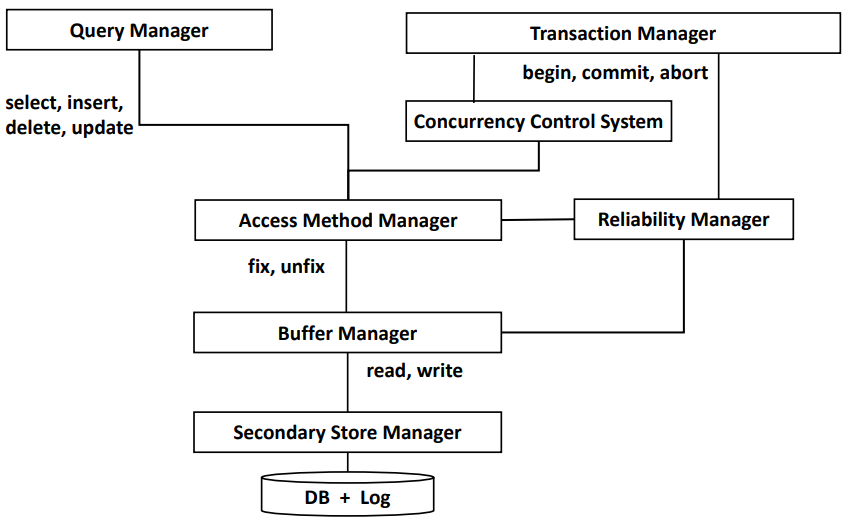
\includegraphics[width=0.75\linewidth]{images/architecture.png}
        \caption{Architecture of a Data Base Management System}
    \end{figure}

\newpage

\chapter{Concurrency}
    \section{Introduction}
    A DBMS usually needs to manage multiple applications. A unit of measurement used to evaluate the DBMS workload is the number of transaction per second (tps) handled by it. 
    To have an efficient usage of the database the DBMS needs to be able to handle concurrency while avoiding the insurgence of anomalies. 
    The concurrency control system schedules the order of the various transactions. 
    
    \section{Anomalies in concurrent transactions}
    The anomalies caused by uncorrect scheduling are: 
    \begin{itemize}
        \item Lost update: an update is applied from a state that ignores a preceding update, which is lost.
            \begin{table}[H]
                \centering
                \begin{tabular}{c|c}
                \textbf{Transaction $t_1$}    & \textbf{Transaction $t_2$} \\ \hline
                $r_1(x)$                      &                            \\
                $x=x+1$                       &                            \\
                                              & $r_2(x)$                   \\
                                              & $x=x+1$                    \\
                                              & $w_2(x)$                   \\
                                              & commit                     \\
                $w_1(x)$                      &                            \\
                commit                        &                           
                \end{tabular}
            \end{table}
        \item Dirty read: an uncommitted value is used to update the data. 
            \begin{table}[H]
                \centering
                \begin{tabular}{c|c}
                \textbf{Transaction $t_1$} & \textbf{Transaction $t_2$} \\ \hline
                $r_1(x)$                   &                            \\
                $x=x+1$                    &                            \\
                $w_1(x)$                   &                            \\
                                        & $r_2(x)$                   \\
                                        & commit                     \\
                abort                      &                           
                \end{tabular}
            \end{table}
        \item Non-repeatable read: someone else updates a previously read value.
            \begin{table}[H]
                \centering
                \begin{tabular}{c|c}
                \textbf{Transaction $t_1$}  & \textbf{Transaction $t_2$} \\ \hline
                $r_1(x)$                    &                            \\
                                            & $r_2(x)$                   \\
                                            & $x=x+1$                    \\
                                            & $w_2(x)$                   \\
                                            & commit                     \\
                $r_1(x)$                    &                            \\
                commit                      & \multicolumn{1}{l}{}      
                \end{tabular}
            \end{table}
        \item Phantom update: someone else updates data that contributes to a previously valid constraint. 
            \begin{table}[H]
                \centering
                \begin{tabular}{c|c}
                \textbf{Transaction $t_1$} & \textbf{Transaction $t_2$} \\ \hline
                $r_1(x)$                   &                            \\
                                           & $r_2(y)$                   \\
                $r_1(y)$                   &                            \\
                                           & $y=y-100$                  \\
                                           & $r_2(z)$                   \\
                                           & $z=z+100$                  \\
                                           & $w_2(y)$                   \\
                                           & $w_2(z)$                   \\
                                           & commit                     \\
                $r_1(z)$                   &                            \\
                $s=x+y+z$                  &                            \\
                commit                     &                           
                \end{tabular}
            \end{table}
        \item Phantom insert: someone else inserts data that contributes to a previously read datum.
    \end{itemize}

    \section{Concurrency theory}
    \begin{definition}
        A \emph{model} is an abstraction of a system, object or process, which purposely disregards details to simplify the investigation of relevant properties. 
    \end{definition}
    Concurrency theory builds upon a model of transaction and concurrency control principles that help understanding the real systems. Real systems exploit implementation level 
    mechanisms which help achieve some desirable properties postulated by the theory. 
    \begin{definition}
        An \emph{operation} consist in a reading or in a writing of a specific datum by a specific transaction. 
    \end{definition}
    \begin{definition}
        A \emph{schedule} is a sequence of operations performed by concurrent transactions that respects the order of operations of each transaction. 
    \end{definition}
    The transactions can be: serial, interleaved or nested. The number of serial schedules for $n$ transaction is equal to 
    \[N_S=n!\]
    While the total number of distinct schedules given the number of transaction $n$ is equal to: 
    \[N_D=\dfrac{\left( \sum_{i=1}^nk_i \right)!}{\prod_{i=1}^n \left( k_i! \right)}\]
    \begin{example}
        Given two transaction $T_1$ and $T_2$ we have six possible different schedules, where only two are serial:
        \begin{enumerate}
            \item $r_1(x) w_1(x) r_2(z) w2(z)$
            \item $r_2(z) w_2(z) r_1(x) w_1(x)$
            \item $r_1(x) r_2(z) w_1(x) w_2(z)$
            \item $r_2(z) r_1(x) w_2(z) w_1(x)$
            \item $r_1(x) r_2(z) w_2(z) w_1(x)$
            \item $r_2(z) r_1(x) w_1(x) w_2(z)$
        \end{enumerate}
        The first two are serial, the third and the fourth are nested, and the last two interleaved.
    \end{example}

    The concurrency control has to reject all the schedules that causes anomalies. 
    \begin{definition}
        The \emph{scheduler} is a component that accepts or rejects operations requested by the transactions. 

        The \emph{serial schedule} is a schedule in which the actions of each transaction occur in a contiguous sequence.
    \end{definition}
    A serializable schedule leaves the database in the same state as some serial schedule of the same transactions, so it is correct. To introduce other classes we have to initially
    make two assumptions: 
    \begin{itemize}
        \item The transactions are observed a posteriori. 
        \item The transactions limited to those that have been committed (commit-projection).
    \end{itemize}

    \section{View-serializability}
    \begin{definition}
        We say that:
        \begin{itemize}
            \item $r_i(x)$ \emph{reads-from} $w_j(x)$ when  $w_j(x)$  precedes  $r_i(x)$ and there is no  $w_k(x)$ in $S$ between  $r_i(x)$  and  $w_j(x)$. 
            \item  $w_i(x)$ in a schedule $S$ is a \emph{final write} if it is the last write on $x$ that occurs in $S$. 
        \end{itemize}

        Two schedules are said to be \emph{view-equivalent} ($S_i \approx_V S_j$) if they have:
        \begin{enumerate}
            \item The same operations. 
            \item The same reads-from relationships.
            \item The same final writes. 
        \end{enumerate}
    \end{definition}

    A schedule is view-serializable (VSR) if it is view-equivalent to a serial schedule of the same transactions.
    The reads-from relationship $r_i(x)$ reads-from $w_j(x)$ in a schedule $S$ assumes that $r_i(x)$ reads the value written by $w_j(x)$ independently of the time at which the 
    commit of $T_j$ occurs. In other words the value written by $w_j(x)$ could be uncommitted when $r_i(x)$ reads it, but we are sure (by definition of commit-projection) that it 
    will be committed.
    \begin{example}
        The following schedules are given:
        \begin{itemize}
            \item $S_1: w_0(x) r_2(x) r_1(x) w_2(x) w_2(z)$
            \item $S_2: w_0(x) r_1(x) r_2(x) w_2(x) w_2(z)$
            \item $S_3: w_0(x) r_1(x) w_1(x) r_2(x) w_1(z)$
            \item $S_4: w_0(x) r_1(x) w_1(x) w_1(z) r_2(x)$
            \item $S_5: r_1(x) r_2(x) w_1(x) w_2(x)$
            \item $S_6: r_1(x) r_2(x) w_2(x) r_1(x)$
            \item $S_7: r_1(x) r_1(y) r_2(z) r_2(y) w_2(y) w_2(z) r_1(z)$
        \end{itemize}
        We have that only $S_2$ and $S_3$ are serial. $S_1$ is view-equivalent to serial schedule $S_2$ (so it is view-serializable). 
        $S_3$ is not view-equivalent to $S_2$ (different operations) but is view-equivalent to serial schedule $S_4$, so it is also view-serializable. 

        $S_5$ corresponds to a lost update, $S_6$ corresponds to a non-repeatable read, and $S_7$ corresponds to a phantom update. All these schedules are non view-serializable. 
        
        The following schedules are given:
        \begin{itemize}
            \item $S_a: w_0(x) r_1(x) w_0(z) r_1(z) r_2(x) w_0(y) r_3(z) w_3(z) w_2(y) w_1(x) w_3(y)$
            \item $S_b: w_0(x) w_0(z) w_0(y) r_2(x) w_2(y) r_1(x) r_1(z) w_1(x) r_3(z) w_3(z) w_3(y)$
            \item $S_c: w_0(x) w_0(z) w_0(y) r_2(x) w_2(y) r_3(z) w_3(z) w_3(y) r_1(x) r_1(z) w_1(x)$
        \end{itemize}
        $S_a$ and $S_b$ are view-equivalent because all the reads-from relationship and final writes are the same. In fact, we have: 
        \begin{itemize}
            \item Reads-from: $r_1(x)$ from $w_0(x)$, $r_1(z)$ from $w_0(z)$, $r_2(x)$ from $w_0(x)$, $r_3(z)$ from $w_0(z)$.
            \item Final writes: $w_1(x)$, $w_3(y)$, $w_3(z)$.
        \end{itemize}
        $S_a$ and $S_c$ are not view-equivalent because not all the reads-from relationship are the same. 
    \end{example}
    Deciding if a generic schedule is in VSR is a NP-complete problem. Therefore, we need to find a stricter definition that is easier to check. The new definition may lead to 
    rejecting some schedule that would be acceptable under view-serializability but not under the stricter/faster criterion.
    
    \section{Conflict-serializability}
    \begin{definition}
        Two operations $o_i$ and $o_j$ ($i \neq j$) are in \emph{conflict} if they address the same resource and at least one of them is a write. There are tho possible cases:
        \begin{enumerate}
            \item Read-write conflicts ($r-w$ or $w-r$).
            \item Write-write conflicts ($w-w$).
        \end{enumerate}

        Two schedules are \emph{conflict-equivalent} (($S_i \approx_C S_j$)) if $S_i$ and $S_j$ contain the same operations and in all the conflicting pairs the transactions occur 
        in the same order. 

        A schedule is \emph{conflict-serializable} (CSR) if and only if it is conflict equivalent to a serial schedule of the same transactions. 
    \end{definition}
    We have that $VSR \subset CSR$ and that $CSR \implies VSR$. 
    \begin{proof}[VSR is a subset of CSR]
        Schedule $S = r_1(x) w_2(x) w_1(x) w_3(x)$ is: 
        \begin{itemize}
            \item View-serializable.
            \item Not conflict-serializable
        \end{itemize}
        It is possible to check that there is no conflict-equivalent serial schedule.
    \end{proof}
    \begin{proof}[CSR implies VSR]
        We assume $S_1 \approx_C S_2$ and prove that $S_1 \approx_V S_2$. $S_1$ and $S_2$ must have: 
        \begin{itemize}
            \item The same final writes: if they didn't, there would be at least two writes in a different order, and since two
                writes are conflicting operations, the schedules would not be $\approx_C$. 
            \item The same reads-from relations: if not, there would be at least one pair of conflicting operations in a different
                order, and therefore, again, $\approx_C$ would be violated. 
        \end{itemize}
    \end{proof}
    The testing of view-serializability is done with a conflict graph that has one node for each transaction $T_i$, and one arc from $T_i$ to $T_j$ if there exists at least one conflict between an operation $o_i$ of $T_i$ and an operation $o_j$ of $T_j$ such that $o_i$ precedes $o_j$.
    \begin{theorem}
        A schedule is in conflict-serializable if and only if its conflict graph is acyclic.
    \end{theorem}
    \begin{example}
        We are given the schedule \[S: w_0(x) r_1(x) w_0(z) r_1(z) r_2(x) w_0(y) r_3(z) w_3(z) w_2(y) w_1(x) w_3(y)\]
        To test the conflict serializability we have to do the following steps: 
        \begin{enumerate}
            \item Create all the nodes based on the number of transactions of the schedule. 
            \item Divide the operation based on resource requested.
            \item Check all the write-write and read-write relationships in each subset, and add the arcs based on these. 
        \end{enumerate}
        In the given example we obtain: 
        \begin{itemize}
            \item $x: w_0 r_1 r_2 w_1$
            \item $y: w_0 w_2 w_3$
            \item $z: w_0 r_1 r_3 w_3$
        \end{itemize}
        \begin{figure}[H]
            \centering
            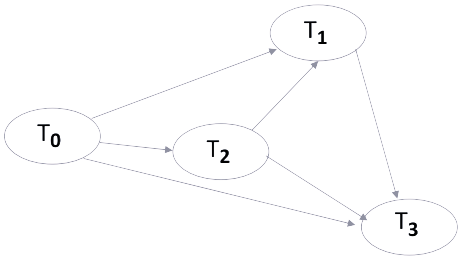
\includegraphics[width=0.5\linewidth]{images/conflict.png}
        \end{figure}
    \end{example}
    \begin{proof}[CSR implies acyclicity of the conflict graph]
        Consider a schedule $S$ in $CSR$. As such, it is $\approx_C$ to a serial schedule. 
        Without loss of generality we can label the transactions of $S$ to say that their order in the serial schedule is: $T_1 T_2 \dots T_n$.
        Since the serial schedule has all conflicting pairs in the same order as schedule $S$, in the conflict graph there can only be arcs $(i,j)$, with $i<j$. 
        Then the graph is acyclic, as a cycle requires at least an arc $(i,j)$ with $i>j$.
    \end{proof}
    \begin{proof}[Acyclicity of the conflict graph implies CSR]
        If $S$'s graph is acyclic then it induces a topological (partial) ordering on its nodes. The same partial order exists on the transactions of $S$. 
        Any serial schedule whose transactions are ordered according to the partial order is conflict-equivalent to $S$, because for all conflicting pairs $(i,j)$ it is always $i<j$. 
    \end{proof}
        
    \section{Concurrency control in practice}
    Conflict-serializability checking would be efficient if we knew the graph from the beginning, but usually we don't. Therefore, a scheduler must rather work online. 
    So, it is not feasible to maintain the conflict graph, update it, and check its acyclicity at each operation request. At the same time, the assumption that concurrency control 
    can work only with the commit-projection of the schedule is unrealistic because aborts do occur. We need some simple on-line decision criterion for the scheduler, which must 
    avoid as many anomalies as possible, and have negligible overhead. 
        
    When dealing with online concurrency control, it is important also to consider arrival sequences. The concurrency control system maps an arrival sequence into an effective a 
    posteriori schedule. To implement this on-line scheduling we use two main families of techniques:
    \begin{itemize}
        \item Pessimistic (locks): if a resource is taken, make the requester wait or pre-empt the holder.
        \item Optimistic (timestamps and versions): serve as many requests as possible, possibly using out-of-date versions of the data. 
    \end{itemize}
    Usually, commercial systems take the best of both worlds. 

    \section{Locking}
    The method called locking is the most used in commercial systems. A transaction is well formed with respect to locking if: 
    \begin{itemize}
        \item Read operations are preceded by $r\_lock$ (shared) and followed by $unlock$. 
        \item Write operations are preceded by $w\_lock$ (exclusive) and followed by $unlock$. 
    \end{itemize}
    In both cases unlocking can be delayed with respect to the end of the read/write operation. So, every object can be: free, r-locked or w-locked. 

    Transactions that first read and then write an object may: acquire a $w\_lock$ already when reading or acquire a $r\_lock$ first and then upgrade it into a $w\_lock$ (escalation).

    The lock manager receives requests from the transactions and grants resources according to the conflict table: 

    \begin{table}[H]
        \centering
        \begin{tabular}{cccc}
        \textbf{}                              & \multicolumn{3}{c}{\textbf{Resource status}}                                                                                                                                                                                                   \\ \cline{2-4} 
        \multicolumn{1}{c|}{\textbf{Request}}  & \multicolumn{1}{c|}{\textit{FREE}}                                          & \multicolumn{1}{c|}{\textit{R\_LOCKED}}                                            & \multicolumn{1}{c|}{\textit{W\_LOCKED}}                                     \\ \hline
        \multicolumn{1}{|c|}{\textit{r\_lock}} & \multicolumn{1}{c|}{\begin{tabular}[c]{@{}c@{}}\checkmark\\ R\_LOCKED\end{tabular}} & \multicolumn{1}{c|}{\begin{tabular}[c]{@{}c@{}}\checkmark\\ R\_LOCKED($n++$)\end{tabular}} & \multicolumn{1}{c|}{\begin{tabular}[c]{@{}c@{}}\tikzxmark\\ W\_LOCKED\end{tabular}} \\ \hline
        \multicolumn{1}{|c|}{\textit{w\_lock}} & \multicolumn{1}{c|}{\begin{tabular}[c]{@{}c@{}}\checkmark\\ W\_LOCKED\end{tabular}} & \multicolumn{1}{c|}{\begin{tabular}[c]{@{}c@{}}\tikzxmark\\ R\_LOCKED\end{tabular}}        & \multicolumn{1}{c|}{\begin{tabular}[c]{@{}c@{}}\tikzxmark\\ W\_LOCKED\end{tabular}} \\ \hline
        \multicolumn{1}{|c|}{\textit{unlock}}  & \multicolumn{1}{c|}{ERROR}                                                  & \multicolumn{1}{c|}{\begin{tabular}[c]{@{}c@{}}\checkmark\\ $n--$\end{tabular}}            & \multicolumn{1}{c|}{\begin{tabular}[c]{@{}c@{}}\checkmark\\ FREE\end{tabular}}      \\ \hline
        \end{tabular}
    \end{table}

    \begin{example}
        Given a schedule with three transactions and the following operations: 
        \[r_1(x)w_1(x)r_2(x)r_3(y)w_1(y)\]
        We have the following locks: 
        \begin{itemize}
            \item $r_1(x)$: $r_1\_lock(x)$ request $\rightarrow$ Ok $\rightarrow$ $x$ is $r-locked$ with $n_x=1$. 
            \item $w_1(x)$: $w_1\_lock(x)$ request $\rightarrow$ Ok $\rightarrow$ $x$ is $w-locked$. 
            \item $r_2(x)$: $r_1\_lock(x)$ request $\rightarrow$ No because $x$ is $w-locked$ $\rightarrow$ $T_2$ waits. 
            \item $r_3(y)$: $r_3\_lock(y)$ request $\rightarrow$ Ok $\rightarrow$ $y$ is $r-locked$ with $n_y=1$ and then $T_3$ unlocks $y$. 
            \item $w_1(y)$: $w_1\_lock(y)$ request $\rightarrow$ Ok $\rightarrow$ $y$ is $w-locked$ and then $x$ and $y$ are freed. 
        \end{itemize}
        So, the schedule a posteriori will became: 
        \[r_1(x)w_1(x)r_3(y)w_1(y)r_2(x)\]
        and we have that the transaction two is delayed. 
    \end{example}
    The locking system is implemented via lock tables, which are hash tables indexing the lockable items via hashing and where each ocked item has a linked list associated with it. 
    Every node in the linked list represents the transaction which requested for lock, lock mode and current status. Every new lock request for the data item is appended as a new 
    node to the list.

    \section{Two-phase locking}
    With the locking showed before we do not eliminate the anomalies caused by non-repeatable reads. To avoid this problem we can use a two-phase rule which requires that a 
    transaction cannot acquire any other lock after releasing a lock. So, we have a phase where the transaction acquires all the locks, a phase where it executes all operations and 
    a fianl phase of unlocking. 
    \begin{definition}
        The class of \emph{two-phase locking} is the set of all schedules generated by a scheduler that: 
        \begin{itemize}
            \item Only processes well-formed transactions. 
            \item Grants locks according to the conflict table. 
            \item Checks that all transactions apply the two-phase rule.             
        \end{itemize}
    \end{definition}
    We have that $2PL \subset CSR \subset VSR$. 
    \begin{proof}[2PL implies CSR]
        We assume that a schedule $S$ is $2PL$. Consider, for each transaction, the end of the plateau (the moment in which it holds all locks and is going to release the first one). 
        We sort the transactions by this temporal value and consider the corresponding serial schedule $S^{'}$. In order to prove (by contradiction) that $S$ is
        conflict-equivalent to $S^{'},S^{'}\approx_CS,\dots$. Consider a generic conflict $o_i \rightarrow o_j$ in $S^{'}$ with $o_i \in T_i$, $0_j \in T_j$, and $i<j$. 
        By definition of conflict, $o_i$ and $o_j$ address the same resource $r$, and at least one of them is a write. The two operations cannot occur in reverse oreder of $S$. 
        This proves that all 2PL schedules are view-serializable too and they can be checked with negligible overhead. 
    \end{proof}
    The anomalies that remains in this state are only the phantom insert (solvable with predicate locks) and the dirty read (requires dealing with abort). 

    \section{Strict two-phase and predicate locking}
    \begin{definition}
        In \emph{strict two-phase locking} (or long duration locks) we also have that locks held by a transaction can be released only after commit or rollback.
    \end{definition}
    This version of locking is used in most commercial DBMS whenever a high level of isolation is required. 

    To prevent phantom inserts a lock should be placed also on future data using the predicate locks. If the predicate lock is on a resource, other transactions cannot insert, delete, 
    or update any tuple satisfying this predicate. 

    \section{Isolation levels in SQL '99}
    SQL defines transaction isolation levels (mainly for read operations) which specify the anomalies that should be prevented by running at that level:
    \begin{itemize}
        \item Read uncommited: allows dirty reads, non-repeatable reads and phantom updates and inserts. No read locks are used. 
        \item Read committed: prevents dirty reads but allows non-repeatable reads and phantom updates/inserts. Normal read locks are used. 
        \item Repeatable read: avoids dirty reads, non-repeatable reads and phantom updates, but allows phantom inserts.  Strict read locks are used. 
        \item Serializable: avoids all anomalies. Strict 2PL with predicate locks are used. 
    \end{itemize}

    \begin{table}[H]
        \centering
        \resizebox{\textwidth}{!}{%
        \begin{tabular}{c|ccc|}
        \cline{2-4}
                                                        & \textbf{Dirty read} & \textbf{Non-repeatable read} & \textbf{Phantoms}    \\ \hline
        \multicolumn{1}{|c|}{\textbf{Read uncommitted}} & $\checkmark$        & $\checkmark$                 & $\checkmark$         \\
        \multicolumn{1}{|c|}{\textbf{Read committed}}   & $\tikzxmark$        & $\checkmark$                 & $\checkmark$         \\
        \multicolumn{1}{|c|}{\textbf{Repeatable reas}}  & $\tikzxmark$        & $\tikzxmark$                 & $\checkmark$(insert) \\
        \multicolumn{1}{|c|}{\textbf{Serializable}}     & $\tikzxmark$        & $\tikzxmark$                 & $\tikzxmark$         \\ \hline
        \end{tabular}%
        }
    \end{table}
    The strictness of serializable level can lead to deadlocks. Therefore, it is not the default in most commercial systems. 
    Transactions requesting locks are either granted the lock or suspended and queued. There is risk of: 
    \begin{itemize}
        \item Deadlock: two or more transactions in endless mutual wait. 
        \item Starvation: a single transaction in endless wait. 
    \end{itemize}

    \section{Deadlocks}
    A deadlock occurs because concurrent transactions hold and in turn request resources held by other transactions. 
    \begin{definition}
        A \emph{lock graph} is a bipartite graph in which nodes are resources or transactions and arcs are lock requests or lock assignments. 

        A \emph{wait-for graph} is a graph in which nodes are transactions and arcs are waits for relationships. 
    \end{definition}
    A deadlock is represented by a cycle in the wait-for graph of transactions. 
    \begin{figure}[H]
        \centering
        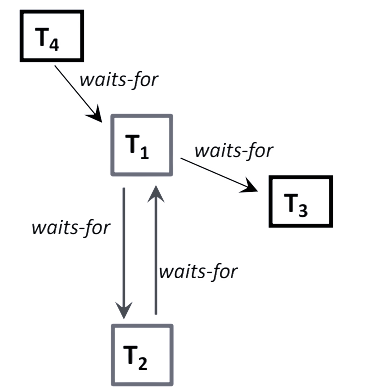
\includegraphics[width=0.35\linewidth]{images/waitgraph.png}
        \caption{An example of deadlock in the wait-for graph}
    \end{figure}
    It is possible to solve deadlocks in three differemt ways: 
    \begin{itemize}
        \item Timeout: a transaction is killed and restarted after a given amount of waiting. The timeout value is system-determined. The problem is choosing a proper timeout value. 
        \item Deadlock prevention: kills transactions that could cause cycles. It is implemented in two ways: 
            \begin{enumerate}
                \item Resource-based prevention puts restrictions on lock requests. The idea is that every transaction requests all resources at once, and only once. The main problem
                    is that it's not easy for transactions to anticipate all requests. 
                \item Transaction-based prevention puts restrictions on transactions' IDs. Assigning IDs to transactions incrementally allows to give an age to each one. It is 
                    possible to choose to kill the holding transaction (preemptive) or the requesting one (non-preemptive). The main problem is the number of killings is too big. 
            \end{enumerate}
        \item Deadlock detection: it can be implemented with Obermarck's algorithm and used for distributed resources. 
    \end{itemize}
    \begin{definition}
        The distributed dependency graph is a wait-for graph where external call nodes represent a sub-transaction activating another sub-transaction at a different node. 
    \end{definition}
    The arrow shows a wait-for relation among local transactions. If one term is an external call, either the source is waited for by a remote transaction or the sink waits for a 
    remote transaction. 
    The Obermarck's algorithm needs the following assumptions: 
    \begin{itemize}
        \item Transactions execute on a single main node. 
        \item Transactions may be decomposed in sub-transactions running on other nodes. 
        \item When a transaction spawns a sub-transaction it suspends work until the latter completes
        \item Two wait-for relationships:
            \begin{itemize}
                \item $T_i$ waits for $T_j$ on the same node because $T_i$ needs a datum locked by $T_j$. 
                \item A sub-transaction of $T_i$ waits for another sub-transaction of $T_i$ running on a different node. 
            \end{itemize}
    \end{itemize}
    The goal of this algorithm is to detect a potential deadlock looking only at the local view of a node using a communication protocol whereby each node has a local projection 
    of the global dependencies. Nodes exchange information and update their local graph based on the received information. Node $A$ sends its local info to a node $B$ only if:
    it contains a transaction $T_i$ that is waited for from another remote transaction and waits for a transaction $T_j$ active on $B$ and $i>j$.
    In other words, I send info to you if a distributed transaction listed at me waits for a distributed transaction listed at you with smaller index. 
    \begin{example}
        Give the following distributed dependency graph: 
        \begin{figure}[H]
            \centering
            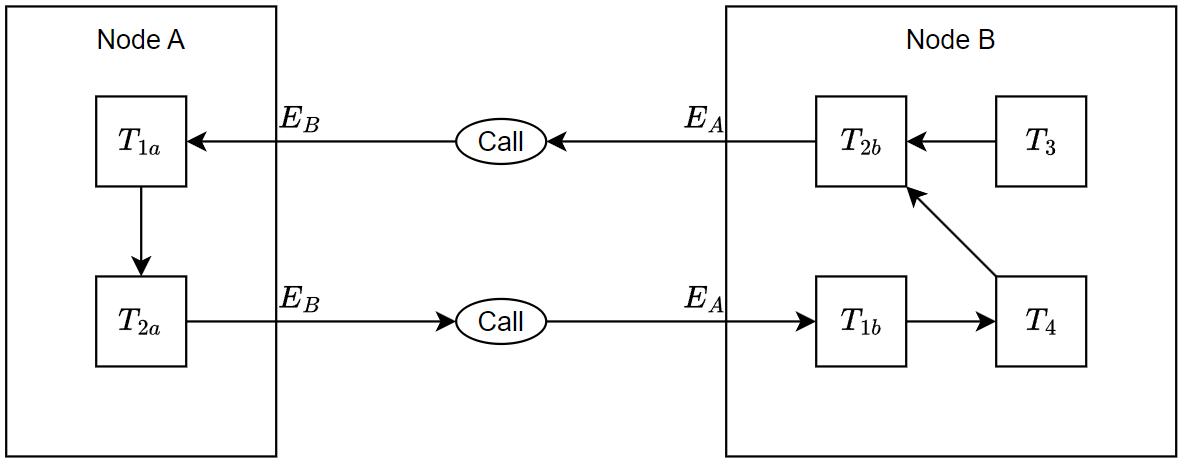
\includegraphics[width=0.5\linewidth]{images/distributedgraph.png}
        \end{figure}
        We can see that the potential deadlock is given by the cycle. In fact, we have that $T_{2a}$ waits for $T_{1a}$ (data lock) that waits for $T_{1b}$ (call) that waits for 
        $T_{2b}$ (data locks) that waits for $T_{2a}$ (call). 
        
        In this case the node $A$ dispatches information to $B$, in fact we have $ E_b \rightarrow T_2 \rightarrow T_1 \rightarrow E_b$ and node $B$ cannot dispatch information to 
        $A$, becasue the forwarding rule is not respected: $E_a \rightarrow T_1 \rightarrow T_2 \rightarrow E_a$. 
    \end{example}
    The Obermarck's algorithm runs periodically at each node and consists in four steps: 
    \begin{enumerate}
        \item Get graph info from the previous nodes.
        \item Update the local graph by merging the received information. 
        \item Check the existence of cycles among transactions denoting potential deadlocks: if found, select one transaction in the cycle and kill it. 
        \item Send updated graph info to the next nodes. 
    \end{enumerate}

\end{document}